\section{Evaluation}
\label{sec:evaluation}

We evaluate \systemname\ on three accelerators with very different
compute-to-bandwidth ratios and three MoE models under a 20\,GB HBM
cap. Throughout, we report two latency components measured by the
instrumentation in \autoref{sec:implementation}: \emph{exposed
waiting} (stall time not overlapped by compute) and \emph{cache-miss
latency} (time spent inside the swap-in path). Compute time is
reported separately and excluded from both. We summarize the headline
findings as follows:

\begin{itemize}[leftmargin=1.4em, itemsep=2pt, topsep=2pt]
    \item \systemname\ reduces the cache-miss latency component
    relative to a fixed-horizon baseline by a geometric mean of
    $\approx 13\times$ across the eight supported model--device pairs,
    while never degrading configurations in which the baseline
    already overlaps most transfers (\autoref{sec:eval:q1}).
    \item Each component contributes independently: the forecaster
    raises prediction accuracy by $21.8\%$ on average (up to
    $30.4\%$, \autoref{sec:eval:predictor}); the two-tier cache
    prevents the eviction--reload cliff that fixed-LRU suffers near
    $S\approx 4$ (\autoref{sec:eval:memory}); cache-aware routing
    suppresses the residual cache-miss component on H20, where
    higher compute throughput exposes more transfer time
    (\autoref{sec:eval:routing}).
    \item Aggregate runtime overhead is below $50\,\mu$s per
    controller update on a commodity CPU, and the forecaster's
    sub-millisecond inference never blocks the GPU critical path
    (\autoref{sec:eval:overhead}).
\end{itemize}

\subsection{Experiment Setup}

\niparagraph{Testbeds.}
All experiments were conducted on three accelerator platforms:
NVIDIA A6000~\cite{nvidiaA6000datasheet} (64~GB/s transfer bandwidth),
NVIDIA H20 (128~GB/s), and Ascend 910B (128~GB/s).
\systemname\ is implemented in Python and CUDA based on the Transformers
framework~\cite{wolf2020transformers}.
To reduce memory fragmentation and enable fine-grained expert residency control,
GPU HBM and host DRAM are managed in block granularity, with dynamic allocation
driven by runtime demand.
Expert swap-in/out transfers are issued on a dedicated CUDA stream to enable
overlap with compute, while a separate CPU thread tracks transfer progress and
memory block states.
We enable continuous batching to emulate serving-style throughput-oriented
execution.

\niparagraph{Workloads and Models.}
Requests are sampled from ShareGPT~\cite{ShareGPT_Vicuna_unfiltered}.
To mitigate heavy-tailed length distribution, we bucket requests by prompt length
and sample up to 50 requests per bucket (within $\pm 5\%$ length variation).
We evaluate three MoE models: DeepSeek-V2-Lite~\cite{DeepSeekCoderV2LiteBase, bi2024deepseek, deepseekai2024deepseekv2strongeconomicalefficient},
Qwen1.5~\cite{Qwen15MoEA27B, qwen_moe}, and Qwen2.0~\cite{Qwen257BA14BInstructGPTQInt4, qwen2}.
We apply INT4 quantization to Qwen2.0 where supported.

\niparagraph{Memory cap and comparability.}
To emulate resource-constrained serving, we cap GPU memory at 20~GB on all
platforms.
This cap forces expert residency competition and makes cache behavior observable.
Ascend 910B currently lacks INT4 support in our software stack, which prevents
running Qwen2.0 under the same 20~GB cap.
We therefore report Qwen2.0 results on A6000 and H20, and report DeepSeek/Qwen1.5
on all three devices.
This limitation is explicitly reflected in tables and does not affect our
cross-device conclusions about the mechanisms of \systemname, which are validated
on two MoE models across all platforms.

\niparagraph{Baselines.}
We compare \systemname\ against a baseline implementation built on Transformers
with representative proactive expert-loading components.
Specifically, the baseline incorporates (i) periodic cross-layer prediction in
the style of ProMoE~\cite{song2024promoe}, and (ii) pregate-based signals commonly
used to approximate upcoming expert activations~\cite{eliseev2023fast}.
We use the term \emph{Baseline} to denote this combined implementation.
When focusing on prediction accuracy alone, we separately report pregate accuracy
and compare against our Predictor (and discuss trend differences relative to
periodic prediction).

\subsection{Q1: Overall Waiting Latency Declines}
\label{sec:eval:q1}

We first evaluate the end-to-end impact of \systemname\ on exposed waiting and
cache-miss latency under memory-capped inference.
Conceptually, \systemname\ reduces waiting by (i) forecasting the experts that will
be needed before execution reaches them, (ii) prefetching these experts early enough
to overlap transfer with compute, and (iii) adapting the forecasting horizon (step
size) to match the current compute--communication ratio and workload dynamics.

\begin{figure*}
    \centering
    \begin{subfigure}{0.32\linewidth}
        \centering
        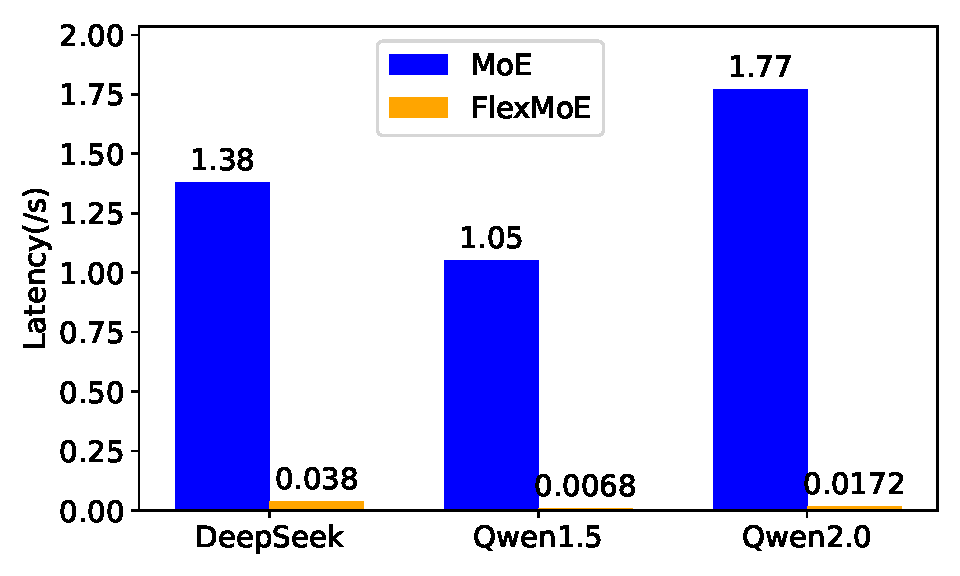
\includegraphics[width=0.99\linewidth]{figures/E2.pdf}
        \caption{NVIDIA A6000}
    \end{subfigure}
    \begin{subfigure}{0.32\linewidth}
        \centering
        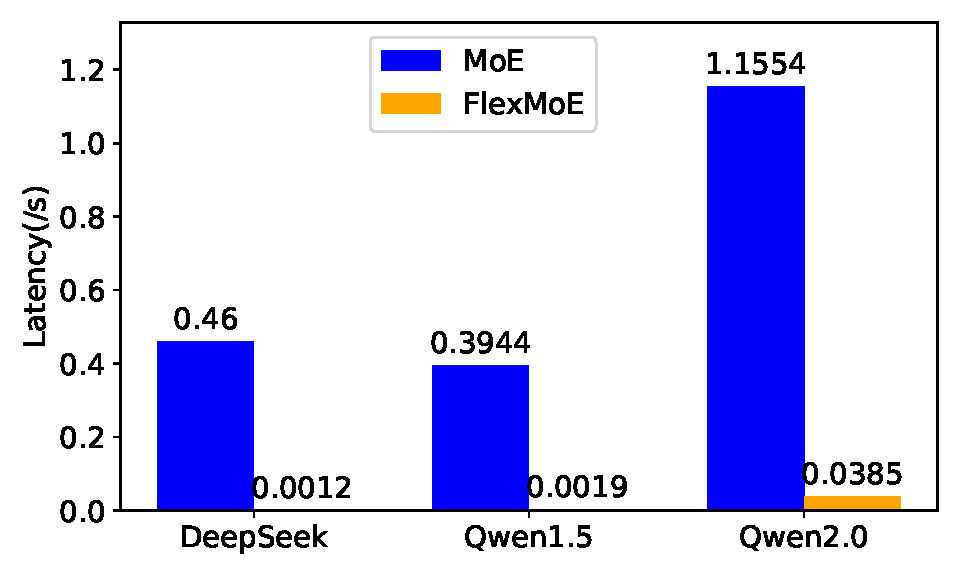
\includegraphics[width=0.99\linewidth]{figures/E2_H20.pdf}
        \caption{NVIDIA H20}
    \end{subfigure}
    \begin{subfigure}{0.32\linewidth}
        \centering
        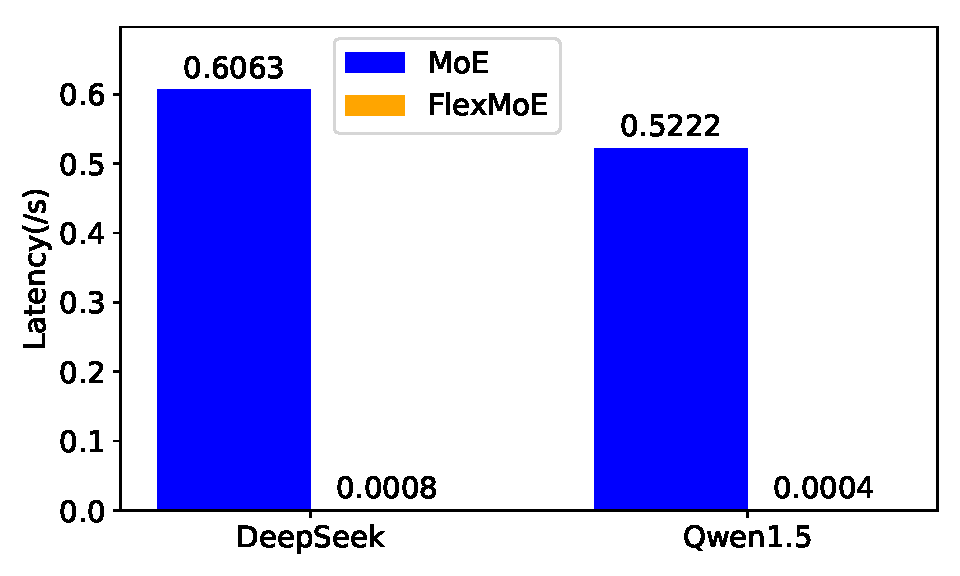
\includegraphics[width=0.99\linewidth]{figures/E2_910B.pdf}
        \caption{Ascend 910B}
    \end{subfigure}
    \caption{Overall waiting + cache-miss latency under memory-capped MoE inference (prompt length 8--1024).}
    \label{fig:E2}
\end{figure*}

We construct a test suite with prompt lengths from 8 to 1024 and
evaluate DeepSeek, Qwen1.5, and Qwen2.0 (where supported).
\autoref{fig:E2} shows that \systemname\ reduces the combined
waiting and cache-miss components relative to the baseline on every
device--model pair. The improvement is consistent across the three
heterogeneous platforms, indicating that \systemname\ adapts to
device-specific overlap opportunities rather than relying on a
single offline-tuned step size. The magnitude of reduction is
largest where expert transfer is on the critical path (Qwen1.5
exhibits the largest gains), and smaller but still positive where
the model already alleviates cache pressure architecturally (Qwen2.0,
whose shared experts~\cite{yang2024qwen2} partially absorb the
problem). Both latency components shrink together, which means
\systemname\ improves overlap without inducing cache thrashing.

A counter-intuitive cross-device data point reinforces the
runtime-control argument. H20's higher peak compute does not always
translate into lower end-to-end latency under our 20\,GB cap: at
small initial~$S$, H20 finishes per-layer compute quickly and then
stalls on transfers because effective bandwidth (and memory-allocator
overhead) does not scale with FLOPs. A6000's slower compute hides a
larger fraction of the same transfer naturally. This is exactly the
brittleness our motivation predicts---the optimal~$S$ shifts with
the compute-to-bandwidth ratio---and \systemname\ converges to
different~$S_t$ on the two devices, recovering the device-specific
overlap opportunity in both.

\subsection{Q2: Pre-Gate-Based Predictor}
\label{sec:eval:predictor}

We next isolate the contribution of the forecaster, since prediction
quality directly affects how often experts are resident when needed
and how much over-prefetch pollutes HBM. The forecaster operates on
token-level features and activation history, so its accuracy is
independent of GPU device; we therefore report it on A6000 as a
representative platform, evaluating 410 requests of varying lengths
under different step numbers when skipping layers in DeepSeek,
Qwen1.5, and Qwen2.0.

\begin{figure}
    \centering
    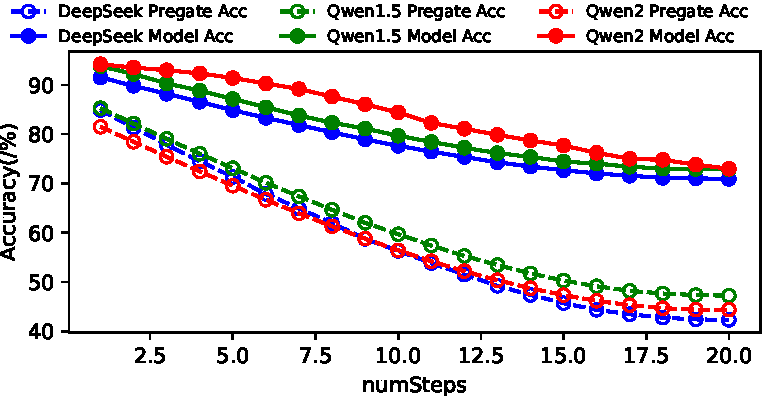
\includegraphics[width=0.99\linewidth]{figures/E1_pregate_model_with_markers.pdf}
    \captionsetup{belowskip=0em,aboveskip=0.0em}
    \vspace{-1.0em}
    \caption{Expert activation prediction accuracy: pregate vs.\ Predictor.}
    \label{fig:predictor-accuracy}
\end{figure}

\autoref{fig:predictor-accuracy} shows that the forecaster improves
accuracy consistently across all three model groups: the average gain
over pregate is $21.79\%$ (up to $30.36\%$). It also degrades more
smoothly as the prediction horizon grows, indicating better robustness
to long-range forecasting than pregate-only signals; compared with
ProMoE-style proactive prediction~\cite{song2024promoe}, the
forecaster achieves higher accuracy at the same step size.

Fitting both accuracy curves to an exponential decay, the asymptotic
accuracy gap $\Delta_\infty$ ranges from 30.8 to 37.0 percentage
points across the three model groups, confirming that the forecaster's
advantage over pregate-only signals is stable at long horizons.

\begin{figure*}[t]
    \centering
    \begin{subfigure}{0.32\linewidth}
        \centering
        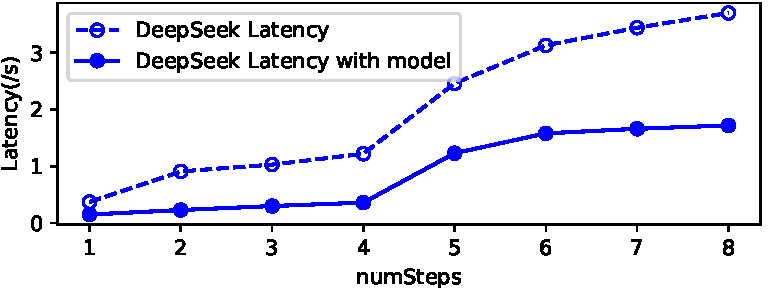
\includegraphics[width=0.99\linewidth]{figures/E1_Group1_Latency.pdf}
        \caption{DeepSeek-V2-Lite}
    \end{subfigure}
    \begin{subfigure}{0.32\linewidth}
        \centering
        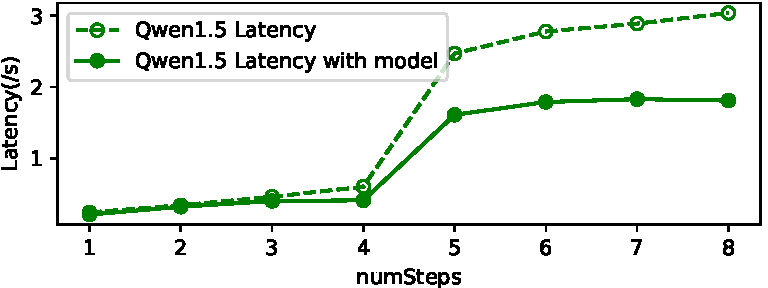
\includegraphics[width=0.99\linewidth]{figures/E1_Group2_Latency.pdf}
        \caption{Qwen1.5-MoE}
    \end{subfigure}
    \begin{subfigure}{0.32\linewidth}
        \centering
        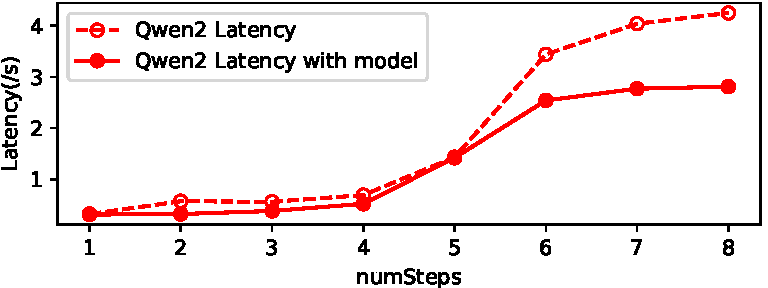
\includegraphics[width=0.99\linewidth]{figures/E1_Group3_Latency.pdf}
        \caption{Qwen2-MoE}
    \end{subfigure}
    \caption{Cache-miss latency after enabling the pregate-based Predictor.}
    \label{fig:E1_latency}
\end{figure*}

Under cross-layer prefetching, prediction errors incur two
complementary costs: under-forecasting misses required experts and
exposes waiting, while over-forecasting loads unused experts,
consuming bandwidth and polluting HBM. Improving prediction accuracy
therefore reduces both components, and \autoref{fig:E1_latency}
confirms this by showing that enabling the forecaster lowers
cache-miss latency across all model groups.

Tables~\ref{tab:Dynamic_baseline}--\ref{tab:Dynamic_predictor}
summarize the cache-miss latency component (seconds per request,
averaged over the 410-request suite at the representative
prompt-length bucket) under the baseline and the forecaster-enabled
configuration; ``--'' denotes a configuration that is unsupported
by the device's software stack under our 20\,GB cap. Values are
means over three runs (per-cell standard deviation $\le 6\%$ of the
mean). The forecaster gives an order-of-magnitude or larger
reduction on every supported configuration except Qwen2-MoE on H20,
where the baseline already overlaps most transfers; the latency
reduction there is correspondingly small but never negative. The
forecaster's robustness to long horizons is what lets the controller
push~$S$ higher when bandwidth is the bottleneck without paying a
misprediction tax.

\begin{table}[t]
\centering
\renewcommand{\arraystretch}{1.2}
\caption{Cache-miss latency (s/request) under the fixed-horizon baseline.}
\label{tab:Dynamic_baseline}
\resizebox{0.9\linewidth}{!}{
\begin{tabular}{c   c   c   c}
\hline\hline
\textbf{Model} & \textbf{A6000} & \textbf{H20} & \textbf{Ascend 910B} \\
\hline
DeepSeek-V2-Lite  & 1.38 & 0.46 & 0.61 \\
Qwen1.5-MoE       & 1.05 & 0.39 & 0.52 \\
Qwen2-MoE         & 1.77 & 1.16 & --   \\ \hline\hline
\end{tabular}
}
\end{table}

\begin{table}[t]
\centering
\renewcommand{\arraystretch}{1.2}
\caption{Cache-miss latency (s/request) with the Predictor enabled.
Reductions are largest where expert transfer dominates the critical
path; on configurations where the baseline already overlaps most
transfers (e.g., Qwen2-MoE on H20) the headroom is smaller, as expected.}
\label{tab:Dynamic_predictor}
\resizebox{0.9\linewidth}{!}{
\begin{tabular}{c   c   c   c}
\hline\hline
\textbf{Model} & \textbf{A6000} & \textbf{H20} & \textbf{Ascend 910B} \\
\hline
DeepSeek-V2-Lite  & 0.044 & 0.001 & 0.062 \\
Qwen1.5-MoE       & 0.038 & 0.038 & 0.069 \\
Qwen2-MoE         & 0.125 & 1.018 & --    \\ \hline\hline
\end{tabular}
}
\end{table}

\subsection{Q2: Memory Management Policy}
\label{sec:eval:memory}

We evaluate the contribution of our memory management policy, which provides
fine-grained control over expert swap operations via an LRU-style residency policy.
The key objective is to prevent pathological eviction--reload cycles that amplify
latency under limited GPU memory.

\begin{figure*}[t]
    \centering
    \begin{subfigure}{0.32\linewidth}
        \centering
        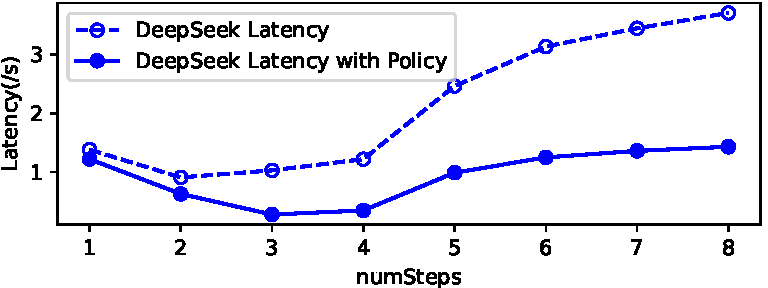
\includegraphics[width=0.99\linewidth]{figures/E3_Group1_Latency.pdf}
        \caption{DeepSeek-V2-Lite}
    \end{subfigure}
    \begin{subfigure}{0.32\linewidth}
        \centering
        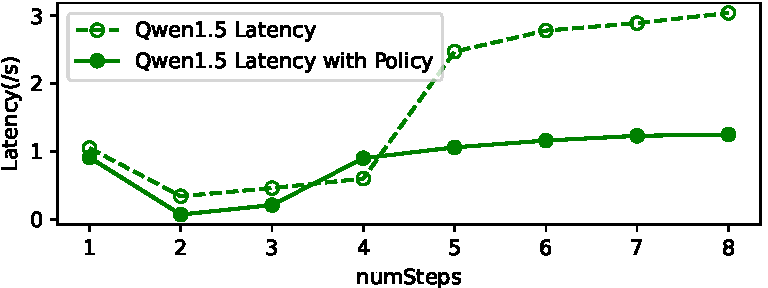
\includegraphics[width=0.99\linewidth]{figures/E3_Group2_Latency.pdf}
        \caption{Qwen1.5-MoE}
    \end{subfigure}
    \begin{subfigure}{0.32\linewidth}
        \centering
        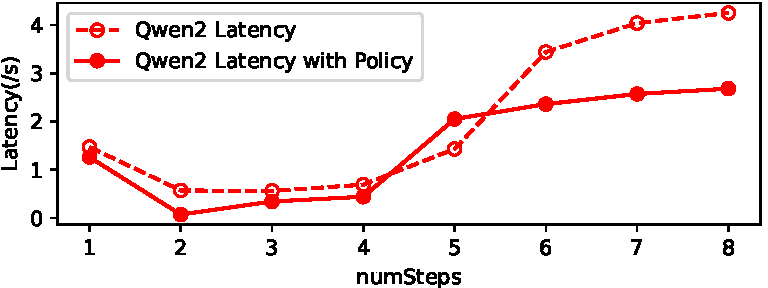
\includegraphics[width=0.99\linewidth]{figures/E3_Group3_Latency.pdf}
        \caption{Qwen2-MoE}
    \end{subfigure}
    \caption{Latency under cross-layer prediction with the proposed memory management policy.}
    \label{fig:E3_latency}
\end{figure*}

\autoref{fig:E3_latency} shows that enabling the two-tier policy
consistently reduces latency compared to the baseline without
dedicated swap-out control. Even with the same forecasting
mechanism, controlling which experts remain resident in HBM is
essential for stabilizing performance under tight memory budgets.
The most informative point is the latency spike that the baseline
exhibits near $S \approx 4$: larger step sizes increase prefetch
depth and short-term residency demand, and once this demand exceeds
the memory cap, eviction--reload cycles amplify latency. The
two-tier residency policy flattens this cliff into a plateau by
localizing the cost of misprediction to a single DMA rather than
triggering an eviction--reload cascade. This is what
makes the controller's exploration of larger~$S$ safe.

\subsection{Q3: Cache-aware Routing}
\label{sec:eval:routing}

Finally, we evaluate cache-aware routing, which couples routing decisions with
current cache residency to reduce cache misses and transfer-induced stalls.
This mechanism is designed to complement both the Predictor and the memory
management policy by reducing the probability that routing selects experts that
are expensive to materialize under current memory pressure.

\begin{figure*}[htp]
    \centering
    \begin{subfigure}{0.32\linewidth}
        \centering
        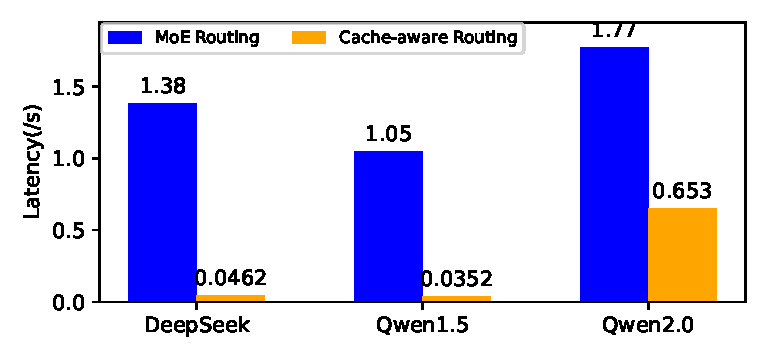
\includegraphics[width=0.99\linewidth]{figures/E4.pdf}
        \caption{NVIDIA A6000}
    \end{subfigure}
    \begin{subfigure}{0.32\linewidth}
        \centering
        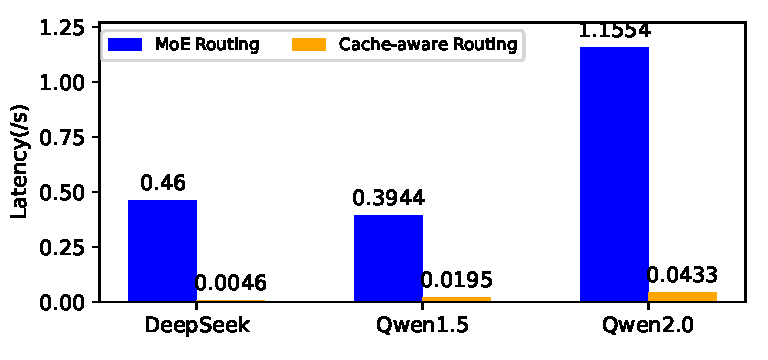
\includegraphics[width=0.99\linewidth]{figures/E4_H20.pdf}
        \caption{NVIDIA H20}
    \end{subfigure}
    \begin{subfigure}{0.32\linewidth}
        \centering
        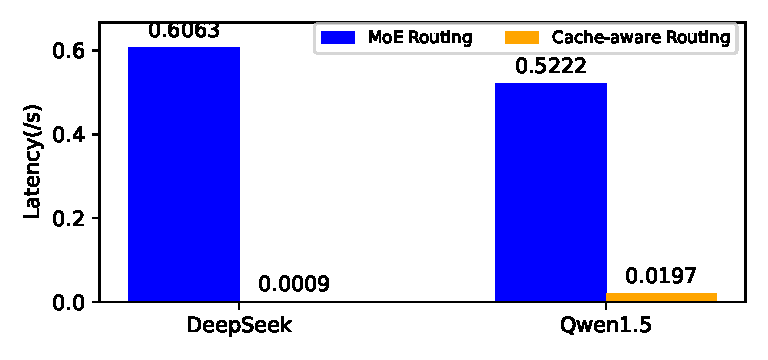
\includegraphics[width=0.99\linewidth]{figures/E4_910B.pdf}
        \caption{Ascend 910B}
    \end{subfigure}
    \caption{End-to-end latency comparison with and without cache-aware routing.}
    \label{fig:cache-aware-routing}
\end{figure*}

\autoref{fig:cache-aware-routing} shows that cache-aware routing
reduces end-to-end latency across DeepSeek, Qwen1.5, and Qwen2.0 by
mitigating expert-loading delays and cache misses. The relative
improvement is strongest for DeepSeek and Qwen1.5, which are more
sensitive to swapping-induced instability under our memory cap.
Qwen2.0 benefits as well, although its built-in shared-expert
design~\cite{yang2024qwen2} already alleviates some cache
inefficiencies; cache-aware routing is therefore complementary
rather than redundant.
\autoref{tab:Dynamic_CCR} reports the cache-miss latency component
(s/request, mean of three runs; same methodology as
Tables~\ref{tab:Dynamic_baseline}--\ref{tab:Dynamic_predictor}) with
cache-aware routing further enabled on top of the forecaster and
the two-tier cache. The largest reduction is on H20, consistent
with its higher compute throughput exposing relatively more transfer
time when routing is cache-oblivious. Combined with the controller
and forecaster, the routing layer closes the loop: prediction errors
that survive the cache no longer propagate into stalls.

\begin{table}[t]
\centering
\renewcommand{\arraystretch}{1.2}
\caption{Cache-miss latency (s/request) with cache-aware routing enabled.}
\label{tab:Dynamic_CCR}
\resizebox{0.9\linewidth}{!}{
\begin{tabular}{c   c   c   c}
\hline\hline
\textbf{Model} & \textbf{A6000} & \textbf{H20} & \textbf{Ascend 910B} \\
\hline
DeepSeek-V2-Lite  & 0.033 & 0.003 & 0.002 \\
Qwen1.5-MoE       & 0.022 & 0.002 & 0.002 \\
Qwen2-MoE         & 0.103 & 0.098 & --    \\ \hline\hline
\end{tabular}
}
\end{table}

\subsection{Runtime Overhead}
\label{sec:eval:overhead}

We separately measure the overhead of the three layers introduced by
\systemname\ to confirm that they do not displace the gains shown in
Q1--Q3. The controller's per-update cost is bounded by \autoref{alg:controller}
to a few EMA updates and a comparison; we measure it at $<50\,\mu$s
on a commodity CPU across all evaluated workloads, which is at least
two orders of magnitude smaller than per-layer compute on every
device. The forecaster runs on the same CPU thread as the
controller; its prediction at control-period granularity is
sub-millisecond and never appears on the GPU critical path, so its
amortized cost is dominated by the per-epoch retraining that runs
between requests. The memory layer's two-tier LRU operates on block
indices and a single asynchronous DMA per eviction, with the
allocator-side cost hidden by the dedicated transfer stream and not
visible in the latency components reported above. Aggregated across
the three layers, the wall-clock overhead introduced by \systemname\
is below the noise floor of our latency-attribution instrumentation,
so the cache-miss reductions in
Tables~\ref{tab:Dynamic_baseline}--\ref{tab:Dynamic_CCR} are net of
all framework costs.

